\section{Sorting}
In this section we will begin our discussion on the implementation of sorting algorithms. Each algorithm contains two variants: a functional and in-place variant. 
The functional variant will return a new list that is sorted, while the in-place variant sorts the list passed as a parameter. 
The functional variant is, in principle, easier to implement, but the in-place variant is more efficient in terms of memory usage. 
Moreover, all lists that are parameters to the sorting algorithms are assumed to be constant-access lists. 
Accordingly, we specify that the input list extends \ttt{AbstractList}\index{\ttt{AbstractList}} class, which guarantees the constant-access property.

For each algorithm, we will assume the same three lists are declared and properly instantiated within the respective unit testing files. 
To conserve space, we enumerate their values below only once.

\begin{verbnobox}[\small]
AbstractList<Integer> LS1 = new ArrayList<>(List.of(5, 4, 2, 1, 3));
AbstractList<Integer> LS2 = new ArrayList<>(List.of());
AbstractList<Integer> LS3 = new ArrayList<>(List.of(10, 8, 6, 7, 2, 10, 3, 3, 3, 10));
\end{verbnobox}

\subsection{Bubble Sort}
Our sorting journey begins with the worst-performing sort out of the five that we will discuss: \emph{bubble sort}\index{bubble sort}. 
With bubble sort, we repeatedly swap adjacent elements if they are in the wrong order. 
We repeat the process until the list is sorted, which is guaranteed after at most~$n^2$ iterations, where~$n$ is the size of the input list. 
Figure~\ref{fig:bubble-sort} illustrates the in-place bubble sort algorithm. 
Note the use of two iteration variables~$i$~and~$j$, where~$i$ represents the outer loop and~$j$ represents the inner loop. 
The inner loop is responsible for the actual swapping of elements, whereas the outer controls the number of traversals over the list. 
The idea is to ``bubble'' the elements to the top/end of the list via repeated comparisons and swapping, hence the name. 
There are optimizations that can be made to the bubble sort algorithm. 
For example, if we traverse through the entire list without swapping at all, then the list must be in sorted order and we can terminate early. 
We will not implement the optimization, but it is worth considering.

\begin{lstlisting}[language=MyJava]
import static Assertions.assertAll;
import static Assertions.assertEquals;

class BubbleSortTester {

  @Test
  void fbs() {
    IBubbleSort<Integer> fbs = new FunctionalBubbleSort<>();
    assertAll(
      () -> assertEquals(List.of(1, 2, 3, 4, 5), 
                         fbs.bubbleSort(LS1)),
      () -> assertEquals(List.of(), 
                         fbs.bubbleSort(LS2)),
      () -> assertEquals(List.of(2, 3, 3, 3, 6, 7, 8, 10, 10, 10), 
                         fbs.bubbleSort(LS3)));
  }

  @Test
  void ipbs() {
    IBubbleSort<Integer> ipbs = new InPlaceBubbleSort<>();
    assertAll(
      () -> ipbs.bubbleSort(LS1),
      () -> assertEquals(List.of(1, 2, 3, 4, 5), LS1),
      () -> ipbs.bubbleSort(LS2),
      () -> assertEquals(List.of(), LS2),
      () -> ipbs.bubbleSort(LS3),
      () -> assertEquals(List.of(2, 3, 3, 3, 6, 7, 8, 10, 10, 10), LS3));
  }
}
\end{lstlisting}

\begin{lstlisting}[language=MyJava]
import java.lang.Comparable;
import java.util.AbstractList;

interface IBubbleSort<V extends Comparable<V>> {
  AbstractList<V> bubbleSort(AbstractList<V> ls);
}
\end{lstlisting}

\subsubsection*{Functional Bubble Sort}
The functional bubble sort removes exactly one instance of the largest element in the list, then recursively sorts the remaining list. Once we know that list is sorted (by the recursive invariant property), we insert the largest element back into the list.

\begin{lstlisting}[language=MyJava]
import java.lang.Comparable;
import java.util.AbstractList;
import java.util.ArrayList;

class FunctionalBubbleSort<V extends Comparable<V>> implements IBubbleSort<V> {

  @Override
  public AbstractList<V> bubbleSort(AbstractList<V> ls) {
    if (ls.size() <= 1) { 
      return ls; 
    } else {
      // Find the largest element.
      V largest = getLargest(ls);
      boolean removed = false;

      // Get all elements but the largest. Removes only
      // one occurrence of the largest element.
      AbstractList<V> rest = new ArrayList<>();
      for (V v : ls) {
        if (v.equals(largest) && !removed) { 
          removed = true; 
        } else { 
          rest.add(v); 
        }
      }

      // Bubble sort the rest, then add the largest as the last element.
      AbstractList<V> newLs = bubbleSort(rest);
      newLs.add(largest);
      return newLs;
    }
  }

  /**
   * Retrieves the largest element in the list. If the list is 
   * empty, null is returned.
   * @param ls the list to search.
   * @return the largest element in the list.
   */
  private V getLargest(AbstractList<V> ls) {
    return ls.stream()
             .max(Comparable::compareTo)
             .orElse(null);
  }
}
\end{lstlisting}

\newpage %ugh
\subsubsection*{In-place Bubble Sort}
\begin{lstlisting}[language=MyJava]
import java.lang.Comparable;
import java.util.AbstractList;
import java.util.Collections;

class InPlaceBubbleSort<V extends Comparable<V>> implements IBubbleSort<V> {

  @Override
  public AbstractList<V> bubbleSort(AbstractList<V> ls) {
    for (int i = 0; i < ls.size(); i++) {
      for (int j = 0; j < ls.size() - i - 1; j++) {
        if (ls.get(j).compareTo(ls.get(j + 1)) > 0) {
          Collections.swap(ls, j, j + 1);
        }
      }
    }
    return ls;
  }
}
\end{lstlisting}

\begin{figure}[tp]
\centering
\begin{tikzpicture}
  % Matrix style
  \tikzset{matrix style/.style={
      matrix of nodes,
      nodes={draw, minimum size=8mm, anchor=center},
      column sep=-\pgflinewidth, row sep=0.1cm,
      nodes in empty cells,
      row 1/.style={nodes={draw=none, minimum size=5mm}},
      column 1/.style={nodes={draw=none, minimum size=5mm}}
  }}

  % Initial list
  \matrix[matrix style] (mat1) {
      \fbox{$i=1$}& 5 & 12 & 98 & 7 & 2 \\
      $j=1$ & |[fill=gray!30]| 5 & |[fill=gray!30]| 12 & 98 & 7 & 2 \\
      $j=2$ & 5 & |[fill=gray!30]| 12 & |[fill=gray!30]| 98 & 7 & 2 \\
      $j=3$ & 5 & 12 & |[fill=gray!30]| 98 & |[fill=gray!30]| 7 & 2 \\
      $j=4$ & 5 & 12 & 7 & |[fill=gray!30]| 98 & |[fill=gray!30]| 2 \\
  };

  % Second iteration of i
  \matrix[matrix style, right=of mat1] (mat2) {
      \fbox{$i=2$}& 5 & 12 & 7 & 2 & 98 \\
      $j=1$ & |[fill=gray!30]| 5 & |[fill=gray!30]| 12 & 7 & 2 & 98 \\
      $j=2$ & 5 & |[fill=gray!30]| 12 & |[fill=gray!30]| 7 & 2 & 98 \\
      $j=3$ & 5 & 7 & |[fill=gray!30]| 12 & |[fill=gray!30]| 2 & 98 \\
      $j=4$ & 5 & 2 & 7 & |[fill=gray!30]| 12 & |[fill=gray!30]| 98 \\
  };

  % Third iteration of i
  \matrix[matrix style, below=of mat1] (mat3) {
      \fbox{$i=3$} & 5 & 2 & 7 & 12 & 98 \\
      $j=1$ & |[fill=gray!30]| 5 & |[fill=gray!30]| 2 & 7 & 12 & 98 \\
      $j=2$ & 2 & |[fill=gray!30]| 5 & |[fill=gray!30]| 7 & 12 & 98 \\
      $j=3$ & 2 & 5 & |[fill=gray!30]| 7 & |[fill=gray!30]| 12 & 98 \\
      $j=4$ & 2 & 5 & 7 & |[fill=gray!30]| 12 & |[fill=gray!30]| 98 \\
  };

  % Fourth iteration of i
  \matrix[matrix style, below=of mat2] (mat4) {
      \fbox{$i=4$}& 2 & 5 & 7 & 12 & 98 \\
      $j=1$ & |[fill=gray!30]| 2 & |[fill=gray!30]| 5 & 7 & 12 & 98 \\
      $j=2$ & 2 & |[fill=gray!30]| 5 & |[fill=gray!30]| 7 & 12 & 98 \\
      $j=3$ & 2 & 5 & |[fill=gray!30]| 7 & |[fill=gray!30]| 12 & 98 \\
      $j=4$ & 2 & 5 & 7 & |[fill=gray!30]| 12 & |[fill=gray!30]| 98 \\
  };
\end{tikzpicture}
\caption{In-Place Bubble Sort Illustration}
\label{fig:bubble-sort}
\end{figure}

\newpage
\subsection{Selection Sort}
The \emph{selection sort}\index{selection sort} is the next sorting algorithm that we will describe. 
Selection sort works by first searching for the smallest element in the list, then swapping it with the first element. 
Then we search for the second smallest element, and swap it with the second element. 
We continue this process until the list is sorted. 
Being that we always search the entire list for the smallest element, this is a horrendously slow sorting algorithm and should be avoided in favor of faster approaches. Nevertheless, we show both the functional and in-place versions. 
Figure~\ref{fig:selection-sort} illustrates the in-place selection sort algorithm. 

\begin{lstlisting}[language=MyJava]
import static Assertions.assertAll;
import static Assertions.assertEquals;

import java.util.List;

class SelectionSortTester {

  @Test
  void fSelSort() {
    ISelectionSort<Integer> ss = new FunctionalSelectionSort<>();
    assertAll(
      () -> assertEquals(List.of(), 
                         ss.selectionSort(LS2)),
      () -> assertEquals(List.of(2, 3, 3, 3, 6, 7, 8, 10, 10, 10), 
                         ss.selectionSort(LS3)));
  }

  @Test
  void ipqsTester() {
    ISelectionSort<Integer> ss = new InPlaceSelectionSort<>();
    assertAll(
      () -> ss.selectionSort(LS2),
      () -> assertEquals(List.of(), LS2),
      () -> ss.selectionSort(LS3),
      () -> assertEquals(List.of(2, 3, 3, 3, 6, 7, 8, 10, 10, 10), LS3));
  }
}
\end{lstlisting}

\begin{lstlisting}[language=MyJava]
import java.lang.Comparable;
import java.util.AbstractList;

interface ISelectionSort<V extends Comparable<V>> {
  AbstractList<V> selectionSort(AbstractList<V> ls);
}
\end{lstlisting}

\newpage
\subsubsection*{Functional Selection Sort}
\begin{lstlisting}[language=MyJava]
import java.util.*;

class FunctionalSelectionSort<V extends Comparable<V>> implements ISelectionSort<V> {

  @Override
  public AbstractList<V> selectionSort(AbstractList<V> ls) {
    if (ls.isEmpty() || ls.size() == 1) { return ls; } 
    else {
      // Recall that min returns an Optional, but we know it is nonempty.
      int minIdx = IntStream.range(0, ls.size())
                            .boxed()
                            .min((i1,i2) -> ls.get(i1).compareTo(ls.get(i2)))
                            .get();

      // Swap the minimum element with the first element.
      Collections.swap(ls, 0, minIdx);
      // Sort the rest of the list (excluding the first element).
      List<V> rest = new ArrayList<>(ls.subList(1, ls.size()));
      AbstractList<V> sortedRest = selectionSort(rest);
      // Construct the final sorted list.
      AbstractList<V> sortedList = new ArrayList<>();
      sortedList.add(ls.get(0));
      sortedList.addAll(sortedRest);
      return sortedList;
    }
  }
}
\end{lstlisting}

% \newpage
\subsubsection*{In-place Selection Sort}
\begin{lstlisting}[language=MyJava]
import java.util.*;

class InPlaceSelectionSort<V extends Comparable<V>> implements ISelectionSort<V> {
  
  @Override
  public AbstractList<V> selectionSort(AbstractList<V> ls) {
    for (int i = 0; i < ls.size(); i++) {
      V min = ls.get(i);
      int minIdx = 0;
      boolean needToSwap = false;
      // Find the minimum value. If we get a value less than the current 
      // minimum, then we need to swap at the end.
      for (int j = i + 1; j < ls.size(); j++) {
        if (ls.get(j).compareTo(min) < 0) {
          min = ls.get(j);
          minIdx = j;
          needToSwap = true;
        }
      }
      if(needToSwap) { Collections.swap(ls, minIdx, i); }
    }
    return ls;
  }
}
\end{lstlisting}  
\begin{figure}[H]
\centering
\begin{tikzpicture}[>=Stealth]
  \matrix (sort) [matrix of nodes, nodes={draw, minimum size=7mm, anchor=center}, column sep=-\pgflinewidth, row sep=0.6cm]{
    $i=0$ & 5 & 2 & 1 & 13 & 98 & 12 & 7 & 6 & 97 \\ % swap 1
    $i=1$ & 1 & 2 & 5 & 13 & 98 & 12 & 7 & 6 & 97 \\ % nothing
    $i=2$ & 1 & 2 & 5 & 13 & 98 & 12 & 7 & 6 & 97 \\ % nothing
    $i=3$ & 1 & 2 & 5 & 13 & 98 & 12 & 7 & 6 & 97 \\ % swap 6
    $i=4$ & 1 & 2 & 5 & 6 & 98 & 12 & 7 & 13 & 97 \\ % swap 7
    $i=5$ & 1 & 2 & 5 & 6 & 7 & 12 & 98 & 13 & 97 \\ % nothing
    $i=6$ & 1 & 2 & 5 & 6 & 7 & 12 & 98 & 13 & 97 \\ % swap 13
    $i=7$ & 1 & 2 & 5 & 6 & 7 & 12 & 13 & 98 & 97 \\ % swap 97
    $i=8$ & 1 & 2 & 5 & 6 & 7 & 12 & 13 & 97 & 98 \\ % nothing
    $i=9$ & 1 & 2 & 5 & 6 & 7 & 12 & 13 & 97 & 98 \\ % nothing
    % $i=8$ & 5 & 2 & 1 & 13 & 98 & 12 & 7 & 6 & 97 \\
    % $i=9$ & 5 & 2 & 1 & 13 & 98 & 12 & 7 & 6 & 97 \\
    % ... other rows can be added for each step
  };

  % Arrows for first swap (5 and 1)
  \draw[->] (sort-1-4.north) |- ++(0,0.5) -| (sort-1-2.north);

  % Do not swap 2.

  % Do not swap 5.

  % Arrows for second swap (6 and 13)
  \draw[->] (sort-4-9.north) |- ++(0,0.5) -| (sort-4-5.north);

  % Arrow for third swap (7 and 98).
  \draw[->] (sort-5-8.north) |- ++(0,0.5) -| (sort-5-6.north);

    % Arrow for third swap (7 and 98).
  \draw[->] (sort-7-9.north) |- ++(0,0.5) -| (sort-7-8.north);
      % Arrow for third swap (7 and 98).
  \draw[->] (sort-8-10.north) |- ++(0,0.5) -| (sort-8-9.north);

  % Arrow for fourth swap (7 down before 12).
  % \draw[->] (sort-6-8.north) |- ++(0,0.5) -| (sort-6-5.north);

  % Arrow for the fifth swap (6 down before 7).
% \draw[->] (sort-7-9.north) |- ++(0,0.5) -| (sort-7-5.north);

  % Arrow for the sixth swap (97 down before 98)
% \draw[->] (sort-8-10.north) |- ++(0,0.5) -| (sort-8-9.north);

    % Red underbars for sorted sublists
\draw[red,thick] (sort-2-2.south west) -- (sort-2-2.south east);
\draw[red,thick] (sort-3-2.south west) -- (sort-3-3.south east);
\draw[red,thick] (sort-4-2.south west) -- (sort-4-4.south east);
\draw[red,thick] (sort-5-2.south west) -- (sort-5-5.south east);
\draw[red,thick] (sort-6-2.south west) -- (sort-6-6.south east);
\draw[red,thick] (sort-7-2.south west) -- (sort-7-7.south east);
\draw[red,thick] (sort-8-2.south west) -- (sort-8-8.south east);
\draw[red,thick] (sort-9-2.south west) -- (sort-9-9.south east);
\draw[red,thick] (sort-10-2.south west) -- (sort-10-10.south east);
  % ... continue this pattern for other rows

  % Additional arrows can be added for other steps
\end{tikzpicture}
\caption{In-Place Selection Sort Illustration}
\label{fig:selection-sort}
\end{figure}

% \newpage
\subsection{Insertion Sort}
The insertion sort is the last of the three poorly-performing sorting algorithms that w will discuss. 
Insertion sort, in general, works by taking an element from the unsorted list and inserting it into the correct position in a sorted list. 
Figure~\ref{fig:insertion-sort} illustrates the in-place insertion sort algorithm; each iteration of the outer loop is represented by a row in the figure, with the red under-bars representing the now-sorted sub-list.

\enlargethispage{-7\baselineskip}
\begin{lstlisting}[language=MyJava]
import static Assertions.assertAll;
import static Assertions.assertEquals;

class InsertionSortTester {

  @Test
  void fInsSort() {
    IInsertionSort<Integer> ss = new FunctionalInsertionSort<>();
    assertAll(
      () -> assertEquals(List.of(1, 2, 3, 4, 5), 
                         ss.insertionSort(LS1)),
      () -> assertEquals(List.of(), 
                         ss.insertionSort(LS2)),
      () -> assertEquals(List.of(2, 3, 3, 3, 6, 7, 8, 10, 10, 10), 
                         ss.insertionSort(LS3)));
  }

  @Test
  void ipInsSort() {
    IInsertionSort<Integer> is = new InPlaceInsertionSort<>();
    assertAll(
      () -> is.insertionSort(LS1),
      () -> assertEquals(List.of(1, 2, 3, 4, 5), LS1),
      () -> is.insertionSort(LS2),
      () -> assertEquals(List.of(), LS2),
      () -> is.insertionSort(LS3),
      () -> assertEquals(List.of(2, 3, 3, 3, 6, 7, 8, 10, 10, 10), LS3));
  }
}
\end{lstlisting}

\begin{lstlisting}[language=MyJava]
import java.util.AbstractList;

interface IInsertionSort<V extends Comparable<V>> {

  AbstractList<V> insertionSort(AbstractList<V> ls);
}
\end{lstlisting}

\newpage
\subsubsection*{Functional Insertion Sort}

The functional insertion sort is a recursive sorting algorithm; it sorts the list by recursively sorting its tail (i.e., the list without the first element). Once the tail is sorted, the algorithm inserts the first element into the sorted tail.
We know how to insert an element into a sorted list: we compare the element to insert with the first element of the sorted list. 
If the list is empty, then we return a list containing only the provided element.
If the element to insert is less than the first element of the sorted list, we insert the element at the beginning of the list, which is provably correct because the list is sorted. 
Otherwise, we (recursively) insert the element into the sorted tail of the list.

\begin{lstlisting}[language=MyJava]
import java.lang.Comparable;
import java.util.AbstractList;
import java.util.ArrayList;

class FunctionalInsertionSort<V extends Comparable<V>> implements IInsertionSort<V> {
  
  @Override
  public AbstractList<V> insertionSort(AbstractList<V> ls) {
    if (ls.isEmpty()) { 
      return new ArrayList<>(); 
    } else { 
      AbstractList<V> rest = (AbstractList<V>) ls.subList(1, ls.size());
      return insert(ls.get(0), insertionSort(rest)); 
    }
  }

  /**
   * Inserts an element into a sorted list of values.
   * @param val value to insert.
   * @param sortedRest a sorted sub-list.
   * @return the sorted sub-list with the new value inserted.
   */
  private AbstractList<V> insert(V val, AbstractList<V> sortedRest) {
    if (sortedRest.isEmpty()) {
      ArrayList<V> ls = new ArrayList<>();
      ls.add(val);
      return ls;
    } else if (val.compareTo(sortedRest.get(0)) < 0) {
      ArrayList<V> ls = new ArrayList<>();
      ls.add(val);
      ls.addAll(sortedRest);
      return ls;
    } else {
      ArrayList<V> ls = new ArrayList<>();
      ls.add(sortedRest.get(0));
      ls.addAll(insert(val, (AbstractList<V>) 
                            sortedRest.subList(1, sortedRest.size())));
      return ls;
    }
  }
}
\end{lstlisting}

\newpage %ugh
\subsubsection*{In-place Insertion Sort}
\begin{lstlisting}[language=MyJava]
import java.lang.Comparable;
import java.util.AbstractList;
import java.util.Collections;

class InPlaceInsertionSort<V extends Comparable<V>> implements IInsertionSort<V> {

  @Override
  public AbstractList<V> insertionSort(AbstractList<V> ls) {
    for (int i = 1; i < ls.size(); i++) {
      V curr = ls.get(i);
      int j = i - 1;
      while (j >= 0 && ls.get(j).compareTo(curr) > 0) {
        Collections.swap(ls, j+1, j);
        j--;
      }
    }
    return ls;
  }
}
\end{lstlisting}

\begin{figure}[ht!]
  \centering
  \begin{tikzpicture}[>=Stealth]
    \matrix (sort) [matrix of nodes, nodes={draw, minimum size=7mm, anchor=center}, column sep=-\pgflinewidth, row sep=0.3cm]{
      $i=1$ & 5 & 2 & 1 & 13 & 98 & 12 & 7 & 6 & 97 \\
      $i=2$ & 2 & 5 & 1 & 13 & 98 & 12 & 7 & 6 & 97 \\
      $i=3$ & 1 & 2 & 5 & 13 & 98 & 12 & 7 & 6 & 97 \\
      $i=4$ & 1 & 2 & 5 & 13 & 98 & 12 & 7 & 6 & 97 \\
      $i=5$ & 1 & 2 & 5 & 13 & 98 & 12 & 7 & 6 & 97 \\
      $i=6$ & 1 & 2 & 5 & 12 & 13 & 98 & 7 & 6 & 97 \\
      $i=7$ & 1 & 2 & 5 & 7 & 12 & 13 & 98 & 6 & 97 \\
      $i=8$ & 1 & 2 & 5 & 6 & 7 & 12 & 13 & 98 & 97 \\
      $i=9$ & 1 & 2 & 5 & 6 & 7 & 12 & 13 & 97 & 98 \\
      % ... other rows can be added for each step
    };
  
    % Arrows for first swap (5 and 2)
    \draw[->] (sort-1-3.north) |- ++(0,0.2) -| (sort-1-2.north west);
  
    % Arrows for second swap (2 and 1)
    \draw[->] (sort-2-4.north) |- ++(0,0.2) -| (sort-2-2.north west);
  
    % Do not swap 13.
  
    % Do not swap 98.
  
    % Arrow for third swap (12 down before 13).
    \draw[->] (sort-5-7.north) |- ++(0,0.2) -| (sort-5-5.north west);
  
    % Arrow for fourth swap (7 down before 12).
    \draw[->] (sort-6-8.north) |- ++(0,0.2) -| (sort-6-5.north west);
  
    % Arrow for the fifth swap (6 down before 7).
  \draw[->] (sort-7-9.north) |- ++(0,0.2) -| (sort-7-5.north west);
  
    % Arrow for the sixth swap (97 down before 98)
  \draw[->] (sort-8-10.north) |- ++(0,0.2) -| (sort-8-9.north west);
  
      % Red under-bars for sorted sub-lists
  \draw[red,thick] (sort-1-2.south west) -- (sort-1-2.south east);
  \draw[red,thick] (sort-2-2.south west) -- (sort-2-3.south east);
  \draw[red,thick] (sort-3-2.south west) -- (sort-3-4.south east);
  \draw[red,thick] (sort-4-2.south west) -- (sort-4-5.south east);
  \draw[red,thick] (sort-5-2.south west) -- (sort-5-6.south east);
  \draw[red,thick] (sort-6-2.south west) -- (sort-6-7.south east);
  \draw[red,thick] (sort-7-2.south west) -- (sort-7-8.south east);
  \draw[red,thick] (sort-8-2.south west) -- (sort-8-9.south east);
  \draw[red,thick] (sort-9-2.south west) -- (sort-9-10.south east);
    % ... continue this pattern for other rows
  
    % Additional arrows can be added for other steps
  \end{tikzpicture}
\caption{In-Place Insertion Sort Illustration}
\label{fig:insertion-sort}
\end{figure}

\newpage
\subsection{Merge Sort}

The \emph{merge sort}\index{merge sort} is one of the first explicitly divide-and-conquer algorithms that programmers encounter. 
We ``divide'' the sorted list into halves, and recursively sort those halves. 
The base case is when the list is either empty or a singleton, since we certainly know how to sort these kinds of lists. 
After dividing comes the ``conquering,'' which consists of taking two now-sorted lists and combining their elements to create yet another sorted list. 
Recall that, at the base case, we know the singletons are sorted by definition. 
Because of this \emph{invariant}\index{invariant}, we know that merging the contents of two sorted lists is not an issue: we compare each element one-by-one, putting the smaller of the two before the subsequent value.

In~\Cref{fig:mergesortill}, we sort the list $[5, 2, 1, 13, 98, 12, 7, 6, 97]$ by decomposing the list into two smaller lists: $[5, 2, 1, 13, 98]$, and $[12, 7, 6, 97]$. 
We recursively decompose these two further until we end with the base case, at which we proceed to merge the now-sorted sub-lists back into one overall sorted list.

\begin{figure}[H]
  \begin{center}
    \begin{tikzpicture}
    \tikzset{every tree node/.style={align=center, anchor=south}, level distance=1.5cm, sibling distance = 0.07cm}
    \scalebox{.90}{
    \Tree 
    [.{\texttt{[5, 2, 13, 98, 12, 7, 6, 97]} (1$\to$8)}
        %LEFT
      [.{\texttt{[5, 2, 13, 98]} (1$\to$4)}
        [.{\texttt{[5, 2]} (1$\to$2)}
            [.{\texttt{[5]} (1)} ]
            [.{\texttt{[2]} (2)} ]
        ]
        [.{\texttt{[13, 98]} (3$\to$4)}
          [.{\texttt{[13]} (4)} ]
          [.{\texttt{[98]} (5)} ]
        ]
      ]
      %RIGHT
      [.{\texttt{[12, 7, 6, 97]}  (5$\to$8)}
        [.{\texttt{[12, 7]} (5$\to$6)}
          [.{\texttt{[12]} (5)} ]
          [.{\texttt{[7]} (6)} ]
        ]
        [.{\texttt{[6, 97]} (7$\to$8)}
          [.{\texttt{[6]} (7)} ]
          [.{\texttt{[97]} (8)} ]
        ]
      ]
    ];
   }
    \end{tikzpicture}
    %REVERSED TREE
    \begin{tikzpicture} [grow'=up]
    \tikzset{every tree node/.style={align=center, anchor=south}, level distance=1.5cm, sibling distance = 0.07cm}
   \scalebox{.90}{
    \Tree 
    [.{\texttt{[2, 5, 6, 7, 12, 13, 97, 98]} (1$\to$8)}
        %LEFT
      [.{\texttt{[2, 5, 13, 98]} (1$\to$4)}
          [.{\texttt{[2, 5]} (1$\to$2)}
            [.{\texttt{[5]} (1)} ]
            [.{\texttt{[2]} (2)} ]
          ]
          [.{\texttt{[13, 98]} (3$\to$4)}
            [.{\texttt{[13]} (3)} ]
            [.{\texttt{[98]} (4)} ]
          ]
      ]
      %RIGHT
      [.{\texttt{[6, 7, 12, 97]} (5$\to$8)}
          [.{\texttt{[7, 12]} (5$\to$6)}
            [.{\texttt{[12]} (5)} ]
            [.{\texttt{[7]} (6)}  ]
          ]
          [.{\texttt{[6, 97]} (7$\to$8)}
            [.{\texttt{[6]} (7)} ]
            [.{\texttt{[97]} (8)} ]
          ]
      ]
    ];
   }
    \end{tikzpicture}
  \end{center}
  \caption{Merge Sort Illustration}
  \label{fig:mergesortill}
\end{figure}

\newpage %ugh
\myexample{Consider merging the lists $l_1 = [9, 11, 14]$, and $l_2 = [2, 20]$.} 
We create a new list~$l_3$ whose size is the sum of the sizes of~$l_1$ and~$l_2$. 
Then, we compare~$9$ against~$2$, of which the latter is smaller, meaning it goes first in~$l_3$. 
Then, we compare~$20$ against~$9$, of which the latter is smaller, meaning it is second. 
Then, we compare~$20$ against~$11$, of which the latter is smaller, meaning it is third. Then, we compare~$20$ against~$14$, of which the latter is, once again, smaller, meaning it is fourth. 
Since we have exhausted all elements of~$l_1$, and we know for certain that~$l_2$ is sorted, we can just copy the remaining elements of~$l_2$ into~$l_3$.

\begin{lstlisting}[language=MyJava]
import static Assertions.assertAll;
import static Assertions.assertEquals;

class MergeSortTester {

  @Test
  void fmsTester() {
    IMergeSort<Integer> ms = new FunctionalMergeSort<>();
    assertAll(
      () -> assertEquals(List.of(1, 2, 3, 4, 5), 
                         ms.mergeSort(LS1)),
      () -> assertEquals(List.of(), 
                         ms.mergeSort(LS2)),
      () -> assertEquals(List.of(2, 3, 3, 3, 6, 7, 8, 10, 10, 10), 
                         ms.mergeSort(LS3)));
  }

  @Test
  void ipmsTester() {
    IMergeSort<Integer> ms = new FunctionalMergeSort<>();
    assertAll(
      () -> ms.mergeSort(LS1),
      () -> assertEquals(List.of(1, 2, 3, 4, 5), LS1),
      () -> ms.mergeSort(LS2),
      () -> assertEquals(List.of(), LS2),
      () -> ms.mergeSort(LS3),
      () -> assertEquals(List.of(2, 3, 3, 3, 6, 7, 8, 10, 10, 10), LS3));
  }
}
\end{lstlisting}
  
\begin{lstlisting}[language=MyJava]
import java.util.AbstractList;

interface IMergeSort<V extends Comparable<V>> {

  AbstractList<V> mergeSort(AbstractList<V> ls);
}
\end{lstlisting}

\newpage %ugh
\subsubsection*{Functional Merge Sort}
\begin{lstlisting}[language=MyJava]
import java.lang.Comparable;
import java.util.AbstractList;
import java.util.ArrayList;
import java.util.List;
  
class FunctionalMergeSort<V extends Comparable<V>> implements IMergeSort<V> {
  
  @Override
  public AbstractList<V> mergeSort(AbstractList<V> ls) { return this.msHelper(ls); }
  
  /**
   * Recursive helper method for merge sort. Splits the list 
   * in half and merges the two halves after recursively sorting them.
   * @param ls the list to sort.
   * @return the sorted list.
   */
  private AbstractList<V> msHelper(AbstractList<V> ls) {
    if (ls.isEmpty()) { return new ArrayList<>(); } 
    else if (ls.size() == 1) {
      AbstractList<V> newLs = new ArrayList<>();
      newLs.add(ls.get(0));
      return newLs;
    } else {
      int mid = (ls.size() - 1) / 2;
      List<V> left = ls.subList(0, mid + 1);
      List<V> right = ls.subList(mid + 1, ls.size());
      AbstractList<V> leftSort = this.msHelper((AbstractList<V>) left);
      AbstractList<V> rightSort = this.msHelper((AbstractList<V>) right);
      return this.merge(leftSort, rightSort);
    }
  }
  
  /**
   * Merges two sorted lists into one sorted list. Compares each 
   * element one-by-one and adds the smaller element to the new list. 
   * If one list is exhausted, the elements of the other list are
   * added to the new list.
   * @param ls1 the first sorted list.
   * @param ls2 the second sorted list.
   * @return the merged sorted list.
   */
  private AbstractList<V> merge(AbstractList<V> ls1, AbstractList<V> ls2) {
    int i, j = 0;
    AbstractList<V> newLs = new ArrayList<>();
    // Merge the lists, comparing the elements.
    while (i < ls1.size() && j < ls2.size()) {
      if (ls1.get(i).compareTo(ls2.get(j)) < 0) { newLs.add(ls1.get(i++)); } 
      else { newLs.add(ls2.get(j++)); }
    }
    // Finish copying ls1.
    while (i < ls1.size()) { newLs.add(ls1.get(i++)); }
    // Finish copying ls2.
    while (j < ls2.size()) { newLs.add(ls2.get(j++)); }
    return newLs;
  }
}
\end{lstlisting}

\subsubsection*{In-place Merge Sort}
\begin{lstlisting}[language=MyJava]
import java.lang.Comparable;
import java.util.AbstractList;
import java.util.ArrayList;

class InPlaceMergeSort<V extends Comparable<V>> implements IMergeSort<V> {

  @Override
  public AbstractList<V> mergeSort(AbstractList<V> ls) {
    this.msHelper(ls, 0, ls.size() - 1);
    return ls;
  }

  /**
   * Recursively sorts the list by splitting it in half and merging the halves.
   * @param ls the list to sort.
   * @param low the lower bound of the sub-list. 
   * @param high the upper bound of the sub-list.
   */
  private void msHelper(AbstractList<V> ls, int low, int high) {
    if (low < high) {
      int mid = low + (high - low) / 2;
      this.msHelper(ls, low, mid);
      this.msHelper(ls, mid + 1, high);
      this.merge(ls, low, mid, high);
    }
  }

  /**
   * Merges two sorted sub-lists into one sorted list. 
   * @param ls the list to sort.
   * @param low the lower bound of the sub-list.
   * @param mid the middle index of the sub-list.
   * @param high the upper bound of the sub-list.
   */
  private void merge(AbstractList<V> ls, int low, int mid, int high) {
    AbstractList<V> ls1 = new ArrayList<>();
    AbstractList<V> ls2 = new ArrayList<>();
    for (int i = low; i <= mid; i++) { ls1.add(ls.get(i)); }
    for (int j = mid + 1; j <= high; j++) { ls2.add(ls.get(j)); }
    int mergeIdx = low;
    int i, j = 0;
    // Merge the elements into the existing list.
    while (i < ls1.size() && j < ls2.size()) {
      if (ls1.get(i).compareTo(ls2.get(j)) < 0) { 
        ls.set(mergeIdx++, ls1.get(i++)); 
      } else { 
        ls.set(mergeIdx++, ls2.get(j++)); 
      }
    }
    // Copy the rest of the elements over.
    while (i < ls1.size()) { ls.set(mergeIdx++, ls1.get(i++)); }
    while (j < ls2.size()) { ls.set(mergeIdx++, ls2.get(j++)); }
  }
}
\end{lstlisting}

\newpage
\subsection{Quick Sort}
At last, we arrive at the \emph{quick sort} algorithm. 
Quick sort works by choosing a \emph{pivot}, which is some value in the list. 
We then recursively sort all elements that are less than the pivot and all those that are greater than the pivot. 
Our implementation of the in-place quicksort works slightly differently, which is why we favor the functional version over the in-place counterpart. 

Quick sort performs optimally when the median is selected as the pivot because roughly half of the elements are less than the pivot and roughly half are greater than the pivot, allowing for a performance similar to that of merge sort. 
Unfortunately, finding the median a priori to sorting ultimately defeats the point. 
In the subsequent chapter, we will analyze the sorting algorithms in more detail.

\begin{lstlisting}[language=MyJava]
import static Assertions.assertAll;
import static Assertions.assertEquals;

class QuickSortTester {

  @Test
  void fqsTester() {
    IQuickSort<Integer> fqs = new FunctionalQuickSort<>();
    assertAll(
      () -> assertEquals(List.of(1, 2, 3, 4, 5), fqs.quicksort(LS1)),
      () -> assertEquals(List.of(), fqs.quicksort(LS2)),
      () -> assertEquals(List.of(2, 3, 3, 3, 6, 7, 8, 10, 10, 10), 
                         fqs.quicksort(LS3)));
  }

  @Test
  void ipqsTester() {
    IQuickSort<Integer> ipqs = new InPlaceQuickSort<>();
    assertAll(
      () -> ipqs.quicksort(LS1),
      () -> assertEquals(List.of(1, 2, 3, 4, 5), LS1),
      () -> ipqs.quicksort(LS2),
      () -> assertEquals(List.of(), LS2),
      () -> ipqs.quicksort(LS3),
      () -> assertEquals(List.of(2, 3, 3, 3, 6, 7, 8, 10, 10, 10), LS3));
  }
}
\end{lstlisting}

\begin{lstlisting}[language=MyJava]
import java.lang.Comparable;
import java.util.AbstractList;

interface IQuickSort<V extends Comparable<V>> {
  AbstractList<V> quicksort(AbstractList<V> ls);
}
\end{lstlisting}

\newpage
\subsubsection*{Functional Quick Sort}
The functional implementation of quick sort is beautiful and elegant. 
We choose a pivot~$p \in L$ at random, then create three sub-lists $l_<$, $l_>$, $l_=$, where~$l_<$ stores all elements less than~$p$, where~$l_>$ stores all elements greater than~$p$, and~$l_=$ stores all elements equal to~$p$. 
Each sub-list, excluding~$l_=$, is recursively sorted, followed by concatenating the three sub-lists in order. 

%%%%%%%%%%%%% FUNCTIONAL QUICK SORT %%%%%%%%%%%%% 
\begin{lstlisting}[language=MyJava]
import java.lang.Comparable;
import java.util.AbstractList;
import java.util.stream.Collectors;

class FunctionalQuickSort<V extends Comparable<V>> 
                          implements IQuickSort<V> {

  @Override
  public AbstractList<V> quicksort(AbstractList<V> ls) {
    if (ls.isEmpty()) { return ls; }
    else {
      // Choose a random pivot.
      V pivot = ls.get((int) (Math.random() * ls.size()));

      // Sort the left-half.
      AbstractList<V> leftHalf = (AbstractList<V>) 
                                  ls.stream()
                                    .filter(x -> x.compareTo(pivot) < 0)
                                    .collect(Collectors.toList());
      AbstractList<V> leftSorted = quicksort(leftHalf);

      // Sort the right-half.
      AbstractList<V> rightHalf = (AbstractList<V>) 
                                   ls.stream()
                                     .filter(x -> x.compareTo(pivot) > 0)
                                     .collect(Collectors.toList());
      AbstractList<V> rightSorted = quicksort(rightHalf);

      // Get all elements equal to the pivot.
      AbstractList<V> equal = (AbstractList<V>) 
                               ls.stream()
                                 .filter(x -> x.compareTo(pivot) == 0)
                                 .collect(Collectors.toList());

      // Merge the three.
      leftSorted.addAll(equal);
      leftSorted.addAll(rightSorted);
      return leftSorted;
    }
  }
}
\end{lstlisting}

%%%%%%%%%%%%% IN PLACE QUICK SORT %%%%%%%%%%%%% 
\newpage
\subsubsection*{In-place Quick Sort}
\begin{lstlisting}[language=MyJava]
import java.lang.Comparable;
import java.util.*;

class InPlaceQuickSort<V extends Comparable<V>> implements IQuickSort<V> {

  @Override
  public AbstractList<V> quicksort(AbstractList<V> ls) {
    this.quicksortHelper(ls, 0, ls.size() - 1);
    return ls;
  }

  /**
   * Recursive helper method for quicksort.
   * @param ls the List to sort.
   * @param low the lower bound of the partition.
   * @param high the upper bound of the partition.
   */
  private void quicksortHelper(AbstractList<V> ls, int low, int high) {
    if (low < high) {
      int pivot = quicksortPartition(ls, low, high);
      quicksortHelper(ls, low, pivot - 1);
      quicksortHelper(ls, pivot + 1, high);
    }
  }

  /**
   * Creates a quicksort partition, where all elements less than 
   * the pivot are to the left of the pivot, and all elements 
   * greater than the pivot are to its right.
   * @param ls the list to partition.
   * @param low the lower bound of the partition.
   * @param high the upper bound of the partition.
   * @return the index of the pivot.
   */
  private int quicksortPartition(AbstractList<V> ls, int low, int high) {
    int rand = new Random().nextInt(high - low + 1) + low;
    Collections.swap(ls, rand, high);
    V pivot = ls.get(high);
    int prevLowest = low;
    for (int i = low; i <= high; i++) {
      if (ls.get(i).compareTo(pivot) < 0) {
        Collections.swap(ls, i, prevLowest++);
      }
    }
    Collections.swap(ls, prevLowest, high);
    return prevLowest;
  }
}
\end{lstlisting}

\newpage
\subsection{Priority Queue Sort}
As a bonus, let's briefly discuss the priority queue sort, which leverages the power of, you guessed it: a priority queue.
Recall from Chapter~\ref{chapter-arrays-collections} that priority queues sort elements based on their priority, which itself is defined as either the natural ordering of the elements or a custom comparator. 
The priority queue sort algorithm works by first adding all elements from the given list into the queue, then repeatedly removing the maximum element from the heap, and placing it at the end of a list. 
Each time an element is polled from the priority queue, its underlying structure is adjusted to reassign the maximum element to the top of the queue.

We create a priority queue from the list, repeatedly poll the queue until it is empty, and add the polled elements to the rear of a new list. 
Remember that inserting elements onto the front of an \ttt{ArrayList} list is slow, so we return a \ttt{LinkedList} instead.\footnote{The other sorting algorithms return instances of \ttt{AbstractList} to guarantee (constant-time) random access to elements. 
The heap sort, on the contrary, will instead return an \ttt{AbstractSequentialList} to ensure that adding elements to the front of the list is constant-time. 
The \ttt{LinkedList} class is a subclass of \ttt{AbstractSequentialList}.}

\begin{lstlisting}[language=MyJava]
import java.lang.Comparable;
import java.util.AbstractSequentialList;
import java.util.List;

interface IPriorityQueueSort<V extends Comparable<V>> {

  AbstractSequentialList<V> pqSort(List<V> ls);
}
\end{lstlisting}

\begin{lstlisting}[language=MyJava]
import java.lang.Comparable;
import java.util.AbstractSequentialList;
import java.util.LinkedList;
import java.util.List;
import java.util.PriorityQueue;
import java.util.Queue;

class FunctionalPriorityQueueSort<V extends Comparable<V>> 
                                  implements IPriorityQueueSort<V> {

  @Override
  public AbstractSequentialList<V> pqSort(List<V> ls) {
    Queue<V> pq = new PriorityQueue<>(ls);
    AbstractSequentialList<V> sorted = new LinkedList<>();
    while (!pq.isEmpty()) {
      sorted.add(pq.poll());
    }
    return sorted;
  }
}
\end{lstlisting}
